\documentclass[11pt]{beamer}
\usetheme{metropolis}

\usepackage[utf8]{inputenc}
\usepackage[romanian,english]{babel}
\usepackage{graphicx}
\usepackage{booktabs}
\usepackage{amsmath}
\usepackage{amsfonts}
\usepackage{tikz}
\usetikzlibrary{positioning, fit, arrows.meta, backgrounds}

% Enable notes (uncomment the line below if you want to print slides with notes)
\setbeameroption{show notes on second screen=right}

\title[Real-Time Quantum-Inspired K-Means]{Real-Time Quantum-Inspired 5D K-Means Image Segmentation}
\subtitle{Sesiunea de Comunicări Științifice ale Studenților}
\author[Sebastian Șoptelea]{Sebastian Șoptelea \\ \vspace{0.2em}{\small Supervisor: Prof. Dr. Anca-Mirela Andreica}}
\institute[UBB]{Faculty of Mathematics and Computer Science \\ Babeș-Bolyai University}
\date[2026]{June 26, 2026}

\begin{document}

% --- Slide 1: Title & Academic Context ---
\begin{frame}
    \titlepage
    \note{
        Hi my name is Sebastian Soptelea and I'm here to present my paper titled Real-time quantum inspired 5D kmeans image segmentation, realised under the supervision of prof. dr anca andreica\\
        This project bridges high-performance GPU programming with quantum-inspired metrics to solve a critical real-time computer vision problem.
    }
\end{frame}

% --- Slide 2: Problem Statement: The Challenge ---
\begin{frame}{Problem Statement: The Challenge}
    \begin{itemize}
        \item \textbf{Core Goal:} Achieving high-fidelity joint color-spatial (5D) image segmentation under strict real-time constraints ($>120$ FPS) for live video.
        \item \textbf{The Segmentation Problem:} Traditional 3D color-only segmentation (e.g., in HSV or BGR) lacks spatial context, leading to highly fragmented regions.
        \item \textbf{5D Joint Manifold ($B,G,R,X,Y$):} Grouping pixels by both color and coordinates preserves spatial consistency, requiring dimension normalization and hardware-level acceleration to handle the computational overhead.
    \end{itemize}
    \note{
        The core goal of this work is achieving high-fidelity joint color-spatial 5D segmentation under strict real-time constraints for live video.\\
        Traditional 3D color-only methods (such as BGR/HSV) lack spatial context, which can lead to highly fragmented regions.\\
        This is why we use a 5D joint manifold which, while it preserves spatial consistency, requires dimension normalization and hardware acceleration to handle the computational overhead.
    }
\end{frame}

% --- Slide 3: Problem Statement: 5D Joint Manifold Mapping ---
\begin{frame}{Problem Statement: 5D Joint Manifold Mapping}
    \begin{figure}[h]
        \centering
        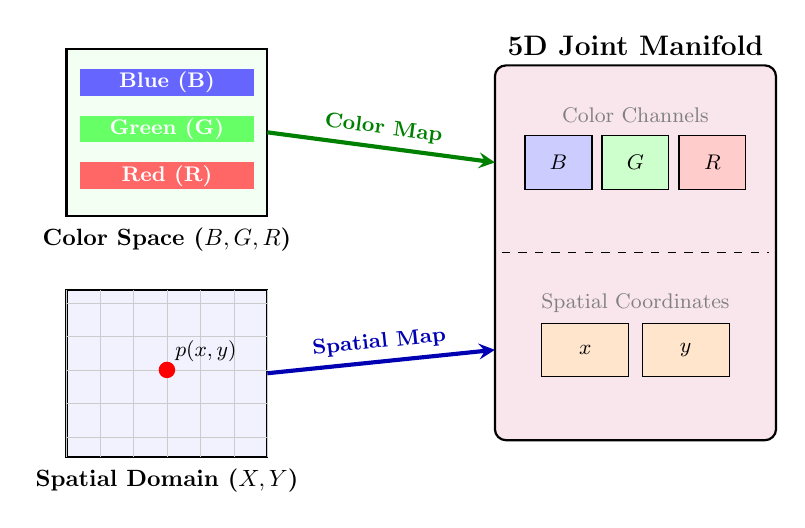
\begin{tikzpicture}[scale=0.85, every node/.style={transform shape}]
            % Color space representation (top-left)
            \draw[thick, fill=green!5] (0,1.8) rectangle (3.0,4.3);
            \draw[fill=blue!60, draw=none] (0.2, 3.6) rectangle (2.8, 4.0);
            \draw[fill=green!60, draw=none] (0.2, 2.9) rectangle (2.8, 3.3);
            \draw[fill=red!60, draw=none] (0.2, 2.2) rectangle (2.8, 2.6);
            \node[font=\small\bfseries, text=white] at (1.5, 3.8) {Blue (B)};
            \node[font=\small\bfseries, text=white] at (1.5, 3.1) {Green (G)};
            \node[font=\small\bfseries, text=white] at (1.5, 2.4) {Red (R)};
            \node[font=\normalsize\bfseries] at (1.5, 1.45) {Color Space ($B, G, R$)};

            % Spatial coordinates representation (bottom-left)
            \draw[thick, fill=blue!5] (0,-1.8) rectangle (3.0,0.7);
            \draw[step=0.5cm, gray!40, very thin] (0,-1.8) grid (3.0,0.7);
            \fill[red] (1.5,-0.5) circle (3.5pt);
            \node[anchor=south west, font=\small\bfseries] at (1.5,-0.5) {$p(x, y)$};
            \node[font=\normalsize\bfseries] at (1.5, -2.15) {Spatial Domain ($X, Y$)};

            % Concat node (right)
            \node (concat) [draw, thick, fill=purple!10, rounded corners, minimum width=4.2cm, minimum height=5.6cm] at (8.5, 1.25) {};
            \node[font=\large\bfseries] at (8.5, 4.35) {5D Joint Manifold};
            
            % Draw components inside concat (top: color) - perfectly centered on x=8.5
            \draw[fill=blue!20] (6.85, 2.2) rectangle (7.85, 3.0) node[pos=.5, font=\small\bfseries] {$B$};
            \draw[fill=green!20] (8.0, 2.2) rectangle (9.0, 3.0) node[pos=.5, font=\small\bfseries] {$G$};
            \draw[fill=red!20] (9.15, 2.2) rectangle (10.15, 3.0) node[pos=.5, font=\small\bfseries] {$R$};
            \node[font=\small, text=gray] at (8.5, 3.3) {Color Channels};
            
            % Draw components inside concat (bottom: spatial) - perfectly centered on x=8.5
            \draw[fill=orange!20] (7.1, -0.6) rectangle (8.4, 0.2) node[pos=.5, font=\small\bfseries] {$x$};
            \draw[fill=orange!20] (8.6, -0.6) rectangle (9.9, 0.2) node[pos=.5, font=\small\bfseries] {$y$};
            \node[font=\small, text=gray] at (8.5, 0.5) {Spatial Coordinates};
            
            \draw[dashed] (6.5, 1.25) -- (10.5, 1.25);
            
            % Connections (no crossing arrows!)
            \draw[->, >=stealth, line width=1.5pt, green!50!black] (3.0, 3.05) -- (6.4, 2.6) node[midway, above, sloped, font=\small\bfseries] {Color Map};
            \draw[->, >=stealth, line width=1.5pt, blue!70!black] (3.0, -0.55) -- (6.4, -0.2) node[midway, above, sloped, font=\small\bfseries] {Spatial Map};
        \end{tikzpicture}
    \end{figure}
    \note{
        To represent this visually, this diagram shows how the joint manifold is structured. For each pixel, we concatenate the three BGR color channels with their corresponding spatial X and Y coordinates to construct a single 5D vector.
    }
\end{frame}

% --- Slide 3: Problem Statement: Requirements \& Bottlenecks ---
\begin{frame}{Problem Statement: Requirements \& Bottlenecks}
    \begin{itemize}
        \item \textbf{Strict Real-Time Requirement (120+ FPS):} Processing budget of $< 8.33$ ms per frame for interactive computer vision (e.g., robotic loops, driving simulators).
        \item \textbf{Hardware Bottlenecks:}
        \begin{itemize}
            \item \emph{CPU Limits:} Sequential 5D clustering requires millions of calculations per frame (too slow for live feeds).
            \item \emph{NISQ QPU Limits:} Real Quantum Processing Units suffer from physical noise, state preparation overhead, and massive network latency.
        \end{itemize}
        \item \textbf{Solution:} A parallel C++/CUDA pipeline that simulates quantum state overlaps directly on local classical GPU cores.
    \end{itemize}
    \note{
        To set the scene, high-speed interactive applications like robotics or driving simulators require a framerate of at least 120 frames per second to avoid latency, giving us a processing budget of under 8.3 milliseconds per frame. Meeting this constraint is challenging because clustering our 5D manifold introduces massive computational overhead, creating a severe bottleneck. Standard CPUs cannot handle these calculations in real time, and physical quantum processors are currently too noisy and slow. This is why we choose to simulate the quantum math locally on a GPU.
    }
\end{frame}

% --- Slide 4: Original Contributions \& What I Bring ---
\begin{frame}{Original Contributions \& What I Bring}
    \begin{itemize}
        \item \textbf{Custom High-Throughput Software Package:} Fully asynchronous CUDA pipeline decoupling the UI from the computational backend.
        \item \textbf{Hardware-Accelerated Quantum Cosine Engine:} Custom kernel utilizing SFU math intrinsics to emulate the SWAP test in real-time.
        \item \textbf{Asynchronous Still-Frame Diagnostics:} On-demand diagnostics on a background thread computing the 3 key quality metrics (WCSS, Davies-Bouldin Index, and Monte Carlo-approximated Silhouette Coefficient) without GUI lag.
        \item \textbf{Two-Tier Atomic Reduction Kernel:} Maximized memory throughput by aggregating sub-totals in block shared memory.
    \end{itemize}
    \note{
        To address these bottlenecks, my work introduces several original contributions. First, I built a fully asynchronous C++/CUDA pipeline that decouples the UI from the computational backend. Second, I developed a custom kernel that utilizes GPU Special Function Unit math intrinsics to emulate the quantum SWAP test in real time. Third, we implemented a non-blocking background thread to run on-demand diagnostics, computing quality metrics like WCSS and Silhouette without lag. Finally, we designed a two-tier atomic reduction kernel to maximize memory throughput.
    }
\end{frame}

% --- Slide 5: System Architecture & Data Pipeline ---
\begin{frame}{System Architecture \& Data Pipeline}
    \begin{itemize}
        \item \textbf{Decoupled Dual-Threaded Model:}
        \begin{itemize}
            \item \emph{UI Thread (Main):} GLFW \& Dear ImGui render loop, rendering segmented OpenGL textures asynchronously.
            \item \emph{Worker Thread:} OpenCV camera capture, preprocessor staging, and active CUDA engine execution.
        \end{itemize}
        \item \textbf{Thread Synchronization Bridge:} Mutex-protected state machine (\texttt{std::scoped\_lock}) preventing race conditions without locking the live rendering pipeline.
        \item \textbf{Memory Efficiency:} Page-locked (pinned) host memory and asynchronous DMA streams (\texttt{cudaMemcpyAsync}) to hide PCIe bus latency.
    \end{itemize}
    \note{
        To achieve the goals mentioned earlier, I developed a system architecture based on a decoupled, dual-threaded model. The main UI thread handles rendering the segmented frames, while a separate worker thread captures camera input and runs the CUDA engine. They communicate asynchronously via a mutex-protected thread synchronization bridge. To hide PCIe bus transfer latency, we employ page-locked host memory and non-blocking, asynchronous CUDA streams.
    }
\end{frame}

% --- Slide 5: System Architecture Diagram ---
\begin{frame}{System Architecture Diagram}
    \begin{figure}[h]
        \centering
        \resizebox{0.98\textwidth}{!}{%
            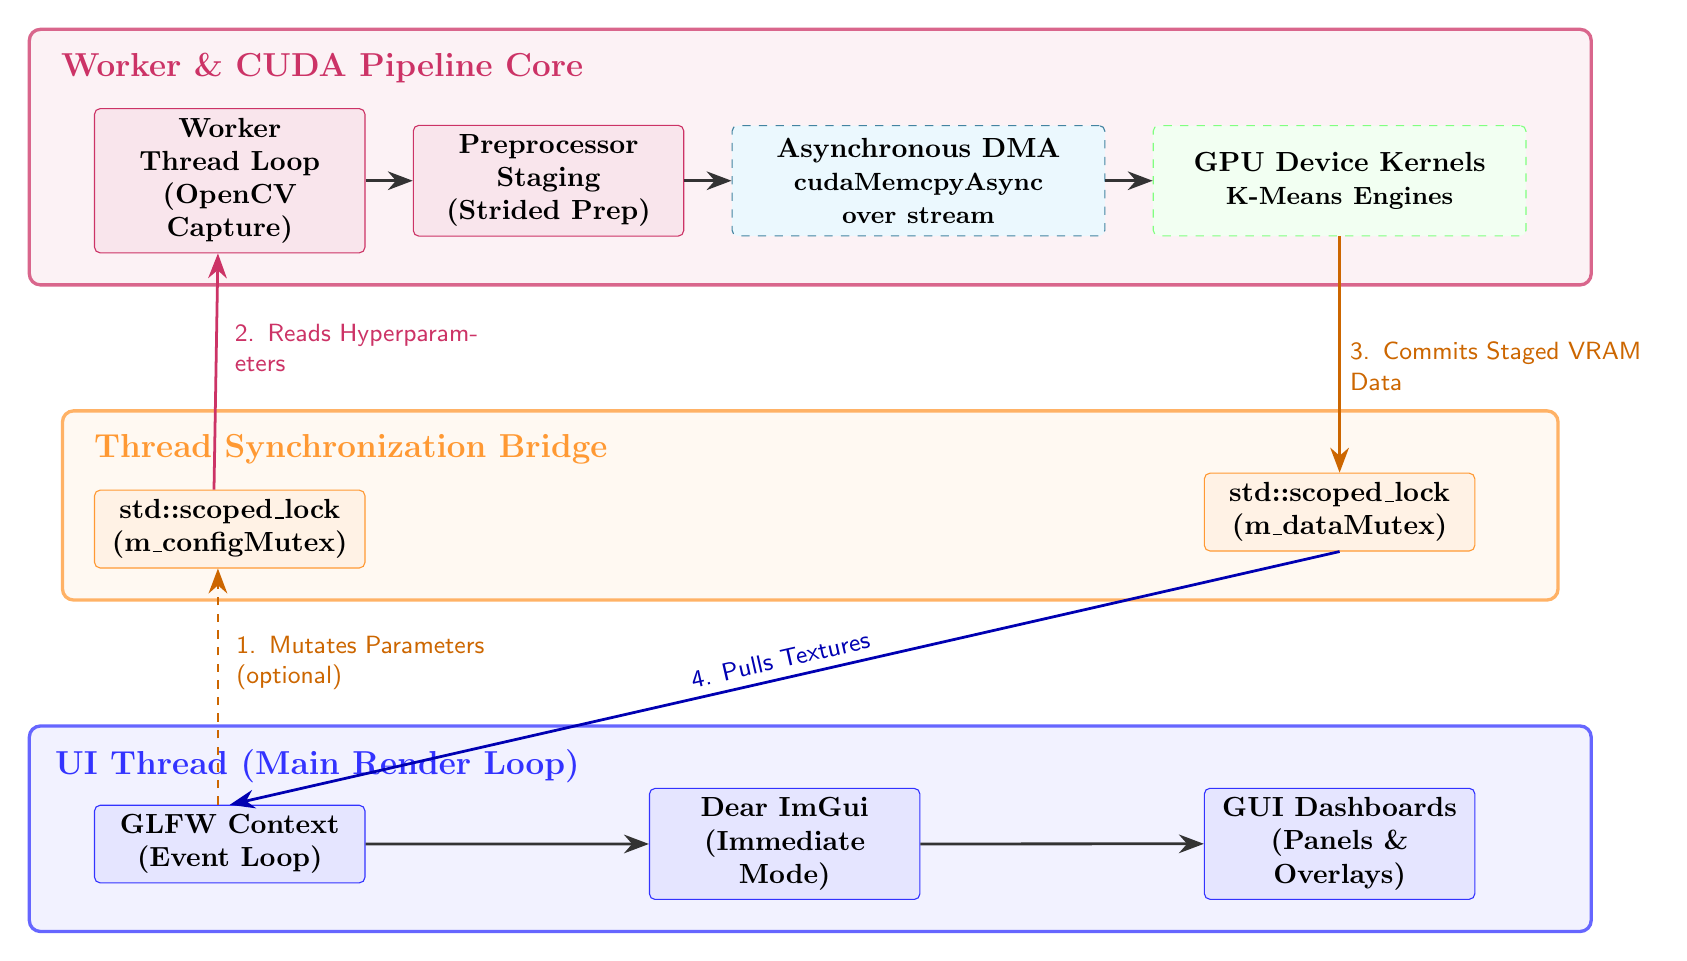
\begin{tikzpicture}[
                node distance = 0.8cm and 0.6cm,
                auto,
                % Box Styles
                layerBox/.style = {rectangle, draw, rounded corners=4, line width=1.2pt, inner sep=0.4cm},
                nodeBox/.style = {rectangle, draw, rounded corners=2, minimum height=0.8cm, fill=white, text width=3.2cm, align=center, font=\normalsize\bfseries},
                subBox/.style = {rectangle, draw, dashed, rounded corners=2, minimum height=1.4cm, text width=4.5cm, align=center, font=\normalsize\bfseries},
                % Arrow Style
                dataLine/.style = {-{Stealth[scale=1.2]}, line width=1pt, draw=black!80}
            ]
                % ==========================================
                % LAYER 1: WORKER & CUDA PIPELINE (TOP PANEL)
                % ==========================================
                \node[nodeBox, fill=purple!10, draw=purple!80] (CV) {Worker Thread Loop \\ (OpenCV Capture)};
                \node[nodeBox, fill=purple!10, draw=purple!80, right=of CV] (Prep) {Preprocessor Staging \\ (Strided Prep)};
                \node[subBox, fill=cyan!8, draw=cyan!60!black, right=of Prep] (DMA) {Asynchronous DMA \\ \small cudaMemcpyAsync over stream};
                \node[subBox, fill=green!5, draw=green!50, right=of DMA] (GPU) {GPU Device Kernels \\ \small K-Means Engines};

                \path[dataLine] (CV) -- (Prep);
                \path[dataLine] (Prep) -- (DMA);
                \path[dataLine] (DMA) -- (GPU);

                % ==========================================
                % LAYER 2: SYNCHRONIZATION BRIDGE (MIDDLE PANEL)
                % ==========================================
                \node[nodeBox, fill=orange!10, draw=orange!80, below=3.0cm of CV] (CfgL) {std::scoped\_lock \\ (m\_configMutex)};
                \node[nodeBox, fill=orange!10, draw=orange!80, below=3.0cm of GPU] (DataL) {std::scoped\_lock \\ (m\_dataMutex)};

                % ==========================================
                % LAYER 3: UI THREAD (BOTTOM PANEL)
                % ==========================================
                \node[nodeBox, fill=blue!10, draw=blue!80, below=3.0cm of CfgL] (GLFW) {GLFW Context \\ (Event Loop)};
                \node[nodeBox, fill=blue!10, draw=blue!80, below=3.0cm of DataL] (Views) {GUI Dashboards \\ (Panels \& Overlays)};
                \path (GLFW.center) -- (Views.center) coordinate[midway] (MidUI);
                \node[nodeBox, fill=blue!10, draw=blue!80] (ImGui) at (MidUI) {Dear ImGui \\ (Immediate Mode)};

                \path[dataLine] (GLFW) -- (ImGui);
                \path[dataLine] (ImGui) -- (Views);

                % Coordinates for container top clearance
                \path (CV.north) ++(0,0.6) coordinate (L1Top);
                \path (CfgL.north) ++(0,0.6) coordinate (L2Top);
                \path (GLFW.north) ++(0,0.6) coordinate (L3Top);

                % ==========================================
                % BACKGROUND CONTAINERS
                % ==========================================
                \begin{pgfonlayer}{background}
                    % Layer 2 first so L1 can reference its extents
                    \node[layerBox, fill=orange!5, draw=orange!60,
                          fit=(CfgL) (DataL) (L2Top)
                              (GPU.south east |- DataL) (CV.south west |- CfgL)] (L2) {};

                    % Layer 1 — forced to match L2's horizontal extents
                    \node[layerBox, fill=purple!5, draw=purple!60,
                          fit=(CV) (GPU) (L1Top)
                              (L2.north west |- CV) (L2.north east |- GPU)] (L1) {};

                    % Layer 3 — forced to match L2's horizontal extents
                    \node[layerBox, fill=blue!5, draw=blue!60,
                          fit=(GLFW) (Views) (ImGui) (L3Top)
                              (L2.south west |- GLFW) (L2.south east |- Views)] (L3) {};
                \end{pgfonlayer}

                % Layer titles
                \node[purple!80, font=\bfseries\large, anchor=north west, xshift=0.3cm, yshift=-0.2cm] at (L1.north west) {Worker \& CUDA Pipeline Core};
                \node[orange!80, font=\bfseries\large, anchor=north west, xshift=0.3cm, yshift=-0.2cm] at (L2.north west) {Thread Synchronization Bridge};
                \node[blue!80, font=\bfseries\large, anchor=north west, xshift=0.225cm, yshift=-0.2cm] at (L3.north west) {UI Thread (Main Render Loop)};

                % ==========================================
                % INTER-LAYER ROUTING LINES
                % ==========================================
                \draw[dataLine, color=orange!80!black, dashed] ([xshift=-0.15cm]GLFW.north) -- ([xshift=-0.15cm]CfgL.south)
                    node[text width=3.2cm, pos=0.6, right, xshift=0.1cm, font=\small\sf] {1. Mutates Parameters (optional)};
                \draw[dataLine, color=purple!80] ([xshift=-0.2cm]CfgL.north) -- ([xshift=-0.15cm]CV.south)
                    node[text width=3.2cm, pos=0.6, right, xshift=0.1cm, font=\small\sf] {2. Reads Hyperparameters};
                \draw[dataLine, color=orange!80!black] (GPU.south) -- (DataL.north)
                    node[text width=3.8cm, pos=0.55, right, font=\small\sf] {3. Commits Staged VRAM Data};
                \draw[dataLine, color=blue!70!black] (DataL.south) -- (GLFW.north)
                    node[sloped, above, pos=0.5, font=\small\sf] {4. Pulls Textures};

            \end{tikzpicture}%
        }
    \end{figure}
    \note{
        To understand how this architecture operates in practice, let's trace the lifecycle of a single video frame processing iteration. First, the UI thread optionally mutates hyperparameters like stride or the cluster count. These are passed through the thread synchronization bridge, where the worker thread reads them. Next, the worker thread handles frame preprocessing and dispatches pixel data to the GPU via asynchronous Direct memory access. Once the GPU completes the segmentation, the processed frame is committed back through the synchronization bridge to the main render loop to update the display.
    }
\end{frame}


% --- Slide 6: Quantum-Inspired Phase-Space Metric ---
\begin{frame}{Quantum-Inspired Phase-Space Metric}
    \begin{itemize}
        \item \textbf{Born's Rule \& The SWAP Test:} Measuring state overlap probability:
        \[ P(|0\rangle) = \frac{1}{2} + \frac{1}{2}|\langle\psi|\phi\rangle|^2 \]
        \item \textbf{Hilbert Phase Space Mapping:}
        \begin{itemize}
            \item Mapping normalized 5D coordinate differences to angular phases in $[0, \frac{\pi}{4}]$:
            \[ \theta_d = |p_d - c_d| \cdot \frac{\pi}{4} \]
            \item Evaluating multi-qubit product state overlaps using squared cosine curves:
            \[ D_{\text{Quantum}}(\mathbf{p},\mathbf{c}) = 1.0 - \prod_{d=1}^{D} \cos^2\left( (p_d - c_d) \cdot \frac{\pi}{4} \right) \]
        \end{itemize}
        \item \textbf{Hardware-Level Emulation:} Compiling trigonometric evaluations into fast, single-cycle device intrinsics (\texttt{\_\_cosf}) executing on the GPU's Special Function Units (SFUs).
    \end{itemize}
    \note{
        Having traced the pipeline's structure, let's examine the quantum-inspired phase-space metric, which is the alternative distance metric introduced in this work. Rather than using traditional Euclidean distance, we measure the overlap probability of two quantum states in Hilbert space, representing a simulation of the SWAP test. We map the normalized 5D coordinate differences to angular phases in the interval $[0, \pi/4]$ and compute their overlap using a product of squared cosines. Because this is computationally expensive, we compile these cosine calculations directly into single-cycle hardware intrinsics executing on the GPU's Special Function Units.
    }
\end{frame}

% --- Slide 7: GPU Kernel \& Memory Optimizations ---
\begin{frame}{GPU Kernel \& Memory Optimizations}
    \begin{itemize}
        \item \textbf{GPU-Native Preprocessor:} Strided preprocessor formatting BGR-XY coordinates into an Array of Structures (AoS), maximizing $L_1$ cache line hit rates and supporting configurable stride-based spatial downsampling.
        \item \textbf{Templated Loop Unrolling:} Forcing compiler branch elimination via 5D templated math utilities (\texttt{\#pragma unroll}) and fast math compiler flags.
        \item \textbf{Two-Tier Atomic Reduction:} A hierarchical aggregation strategy (detailed in the next slide) designed to minimize global memory traffic bottlenecks.
    \end{itemize}
    \note{
        To run this quantum emulation in real time, I implemented several hardware-level GPU optimizations. First, the GPU-native preprocessor formats pixel data into an Array of Structures to maximize L1 cache hit rates, while also handling spatial downsampling using a configurable stride parameter. Second, we use templated vector math and compiler pragmas to force complete loop unrolling and eliminate branching. Finally, we address the global memory writeback bottleneck using a two-tier atomic reduction kernel, which we will detail in the next slide.
    }
\end{frame}

% --- Slide 8: Two-Tier Atomic Reduction ---
\begin{frame}{Two-Tier Atomic Reduction}
    \begin{figure}[h]
        \centering
        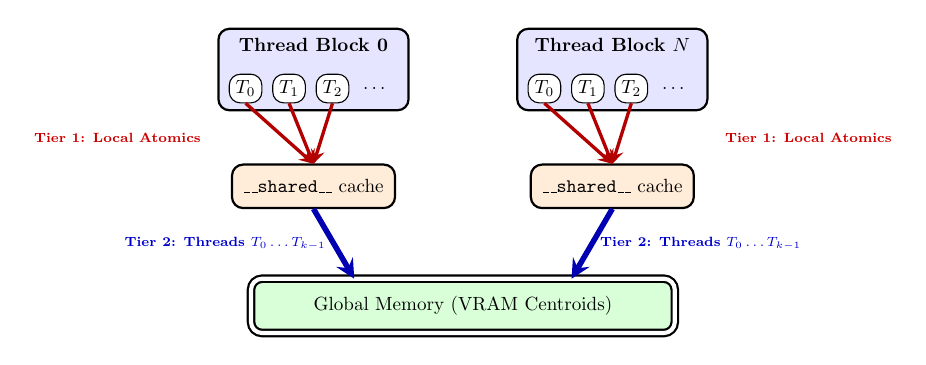
\begin{tikzpicture}[scale=0.69, every node/.style={transform shape}]
            % Threads Block 0
            \draw[thick, fill=blue!10, rounded corners] (0, 3) rectangle (3.5, 4.5);
            \node[font=\bfseries] at (1.75, 4.2) {Thread Block 0};
            \node (t0) [draw, fill=white, rounded corners, minimum width=0.6cm] at (0.5, 3.4) {$T_0$};
            \node (t1) [draw, fill=white, rounded corners, minimum width=0.6cm] at (1.3, 3.4) {$T_1$};
            \node (t2) [draw, fill=white, rounded corners, minimum width=0.6cm] at (2.1, 3.4) {$T_2$};
            \node at (2.9, 3.4) {\dots};

            % Threads Block N
            \draw[thick, fill=blue!10, rounded corners] (5.5, 3) rectangle (9, 4.5);
            \node[font=\bfseries] at (7.25, 4.2) {Thread Block $N$};
            \node (tN0) [draw, fill=white, rounded corners, minimum width=0.6cm] at (6.0, 3.4) {$T_0$};
            \node (tN1) [draw, fill=white, rounded corners, minimum width=0.6cm] at (6.8, 3.4) {$T_1$};
            \node (tN2) [draw, fill=white, rounded corners, minimum width=0.6cm] at (7.6, 3.4) {$T_2$};
            \node at (8.4, 3.4) {\dots};

            % Shared Memory Block 0
            \node (sh0) [draw, thick, fill=orange!15, minimum width=3cm, minimum height=0.8cm, rounded corners] at (1.75, 1.6) {\texttt{\_\_shared\_\_} cache};
            % Shared Memory Block N
            \node (shN) [draw, thick, fill=orange!15, minimum width=3cm, minimum height=0.8cm, rounded corners] at (7.25, 1.6) {\texttt{\_\_shared\_\_} cache};

            % Global VRAM
            \node (vram) [draw, double, double distance=1.5pt, thick, fill=green!15, minimum width=7.8cm, minimum height=1.0cm, rounded corners] at (4.5, -0.6) {Global Memory (VRAM Centroids)};

            % Arrows Tier 1
            \draw[->, >=stealth, line width=1.2pt, red!70!black] (t0.south) -- (sh0.north);
            \draw[->, >=stealth, line width=1.2pt, red!70!black] (t1.south) -- (sh0.north);
            \draw[->, >=stealth, line width=1.2pt, red!70!black] (t2.south) -- (sh0.north);

            \draw[->, >=stealth, line width=1.2pt, red!70!black] (tN0.south) -- (shN.north);
            \draw[->, >=stealth, line width=1.2pt, red!70!black] (tN1.south) -- (shN.north);
            \draw[->, >=stealth, line width=1.2pt, red!70!black] (tN2.south) -- (shN.north);

            % Arrows Tier 2
            \draw[->, >=stealth, line width=2pt, blue!70!black] (sh0.south) -- (2.5, -0.1) node[midway, left, font=\scriptsize\bfseries, text=blue!80!black] {Tier 2: Threads $T_0 \dots T_{k-1}$};
            \draw[->, >=stealth, line width=2pt, blue!70!black] (shN.south) -- (6.5, -0.1) node[midway, right, font=\scriptsize\bfseries, text=blue!80!black] {Tier 2: Threads $T_0 \dots T_{k-1}$};

            % Tier 1 Labels (moved to the sides to avoid arrow crossing)
            \node[font=\scriptsize\bfseries, text=red!80!black, left] at (-0.2, 2.5) {Tier 1: Local Atomics};
            \node[font=\scriptsize\bfseries, text=red!80!black, right] at (9.2, 2.5) {Tier 1: Local Atomics};

        \end{tikzpicture}
    \end{figure}
    \begin{itemize}
        \item \textbf{Tier 1 (Block Atomics):} GPU threads accumulate coordinate sub-totals locally inside fast on-chip shared memory, avoiding costly global memory bus traffic.
        \item \textbf{Tier 2 (Global Atomics):} The first $K$ threads per block ($T_0 \dots T_{k-1}$) flush the accumulated sub-totals to Global VRAM, parallelizing the final reduction.
    \end{itemize}
    \note{
        Looking at this two-tier atomic reduction diagram, we can see exactly how the memory bottleneck is resolved. In Tier 1, all threads accumulate cluster coordinate sums and pixel counts locally inside the fast, on-chip shared memory of their block using block atomics, which dramatically cuts down global bus traffic. Then, in Tier 2, only the first $K$ threads per block—from $T_0$ to $T_{k-1}$—flush these pre-aggregated sums and counts to the global VRAM centroid arrays in parallel. Because the block size is 256, this two-tier structure reduces global memory contention by 256 times. These final values are then used to compute the updated cluster centroids, which ultimately determine which pixels get assigned to each cluster and how they are colored.
    }
\end{frame}


% --- Slide 9: Experimental Results \& Telemetry ---
\begin{frame}{Experimental Results \& Telemetry}
    \begin{table}[h]
        \centering
        \footnotesize
        \begin{tabular}{cccccc}
            \toprule
            \multicolumn{2}{c}{\textbf{Configuration}} & \multicolumn{2}{c}{\textbf{Classical Engine}} & \multicolumn{2}{c}{\textbf{Quantum Engine}} \\
            \cmidrule(r){1-2} \cmidrule(lr){3-4} \cmidrule(l){5-6}
            \textbf{$K$ (Clusters)} & \textbf{$S$ (Stride)} & \textbf{Latency} & \textbf{Iterations} & \textbf{Latency} & \textbf{Iterations} \\
            \midrule
            3  & 8  & 1.81 ms  & 11.71  & 1.61 ms  & 12.38  \\
            8  & 4  & 6.45 ms  & 41.81  & 6.15 ms  & 41.43  \\
            40 & 1  & 26.66 ms & 88.67  & 27.95 ms & 88.62  \\
            \bottomrule
        \end{tabular}
    \end{table}
    
    \begin{itemize}
        \item \textbf{Speed Parity:} Dedicated GPU Special Function Units (SFUs) execute simulated trigonometric distances in a single clock cycle, maintaining latency parity with the Euclidean solver.
        \item \textbf{Functional Equivalence:} Although not listed in the table, all diagnostic quality metrics (WCSS, Davies-Bouldin Index, and Silhouette Coefficient) are mathematically identical across both backends.
    \end{itemize}
    \note{
        These hardware optimizations translate directly into the performance telemetry shown in this benchmark table. As you can see, the quantum-inspired engine maintains complete speed parity with the classical Euclidean baseline. For example, with $K=3$ and a stride of 8, both run in under 1.8 milliseconds. This confirms that compiling the quantum metric's trigonometric evaluations into fast, single-cycle Special function unit instructions prevents any computational overhead. Furthermore, all quality metrics like within cluster sum of squares and Davies-Bouldin are mathematically identical across both solvers, confirming their functional equivalence.
    }
\end{frame}

% --- Slide 10: Visual Segmentation Comparison ---
\begin{frame}{Visual Segmentation Comparison}
    \begin{columns}
        \begin{column}{0.32\textwidth}
            \centering
            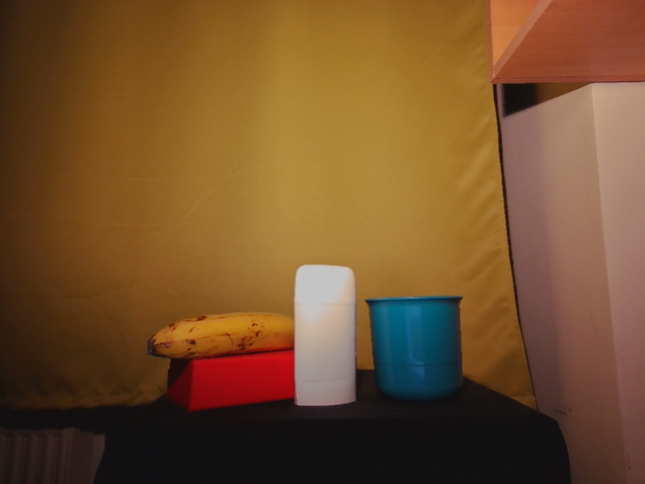
\includegraphics[width=\textwidth]{../thesis/figures/scene_a.png}
            \vskip 0.3em
            {\small Original Image}
        \end{column}
        \begin{column}{0.32\textwidth}
            \centering
            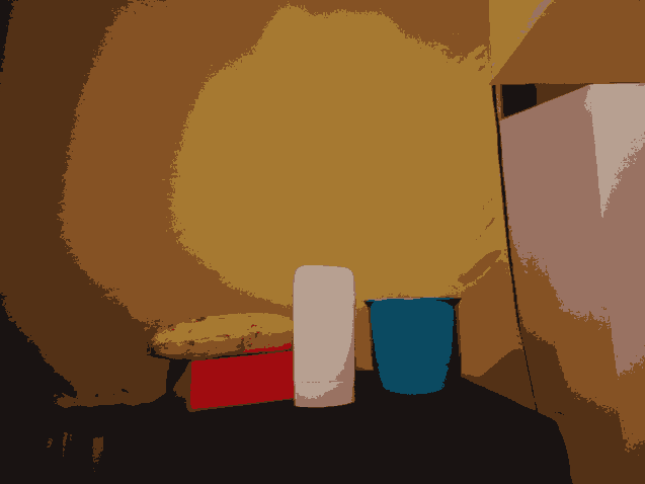
\includegraphics[width=\textwidth]{../thesis/figures/scene_a_classical.png}
            \vskip 0.3em
            {\small Classical Euclidean}
        \end{column}
        \begin{column}{0.32\textwidth}
            \centering
            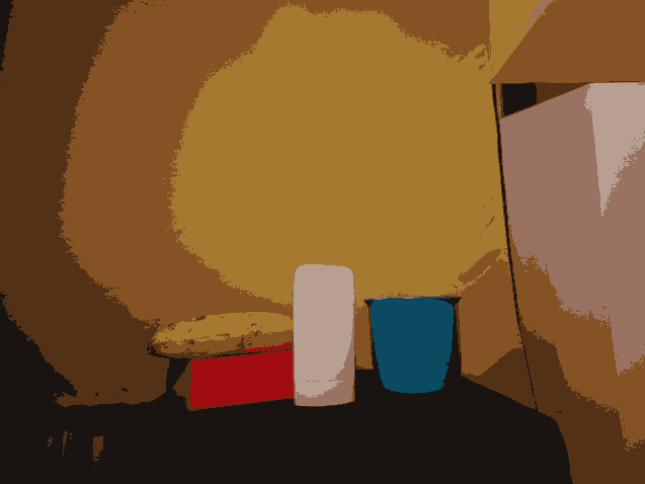
\includegraphics[width=\textwidth]{../thesis/figures/scene_a_quantum.png}
            \vskip 0.3em
            {\small Quantum-Inspired}
        \end{column}
    \end{columns}
    
    \vspace{0.8em}
    \begin{itemize}
        \item \textbf{Visual Parity:} Both solvers produce visually identical cluster assignments, confirming the functional correctness of the phase-space mapping.
    \end{itemize}
    \note{
        Here we can see a side-by-side visual comparison of the segmentation output. The original image on the left is segmented into identical spatial color clusters by both the classical Euclidean engine in the middle and the quantum-inspired engine on the right. Because the quantum phase distance is a monotonic mapping of feature similarity, it yields identical convergence states and final metrics. This demonstrates and validates the complete functional correctness of our quantum emulation.
    }
\end{frame}

% --- Slide 12: Conclusions ---
\begin{frame}{Conclusions}
    \begin{itemize}
        \item \textbf{High-Throughput Pipeline:} Developed a decoupled, multi-threaded C++/CUDA 5D image segmentation pipeline achieving over 120 FPS.
        \item \textbf{Algorithmic Parity:} Proved exact functional, visual, and mathematical convergence parity between the quantum-inspired and classical solvers.
        \item \textbf{Zero Performance Overhead:} Demonstrated that quantum-inspired distance metrics (simulating state overlaps) can be simulated efficiently on local GPU hardware via SFU intrinsics (\texttt{\_\_cosf}).
    \end{itemize}
    \note{
        To conclude, I would like to summarize our main findings. First, we successfully developed a decoupled, multi-threaded C++/CUDA pipeline that comfortably exceeds our 120 FPS real-time target. Second, we proved exact functional, visual, and mathematical convergence parity between the quantum-inspired solver and the classical baseline. Finally, we demonstrated that emulating quantum state overlaps in Hilbert space introduces zero performance overhead because these calculations are compiled directly into fast, single-cycle GPU hardware intrinsics on the Special Function Units.
    }
\end{frame}

% --- Slide 13: Publications \& Academic Activity ---
\begin{frame}{Publications \& Academic Activity}
    \vfill
    \begin{itemize}
        \item \textbf{Book Chapter (HAIS 2026):} \\
        {\footnotesize Şoptelea, S., Kallay, P., Tudor, M., Lung, R.I. (2027). \emph{A Variational Quantum Classifier Applied to Romanian Financial Data}. In: Hybrid Artificial Intelligent Systems. Lecture Notes in Computer Science, vol 16596, pp. 429–440. Springer, Cham. DOI: 10.1007/978-3-032-29292-6\_35.}
        \item \textbf{Ongoing Research:} A comprehensive Quantum Machine Learning (QML) literature survey in the works.
    \end{itemize}
    \vfill
    \note{
        In addition to the core findings of this thesis, I would like to highlight my related academic work. This research was inspired by my first-author book chapter published in Springer for HAIS 2026, which applied variational quantum classifiers to Romanian financial data. Building on these concepts, I also have an ongoing comprehensive Quantum Machine Learning literature survey in preparation.
    }
\end{frame}

% --- Slide 14: Future Work ---
\begin{frame}{Future Work}
    \begin{itemize}
        \item \textbf{Spatiotemporal Tracking:} Integrating temporal continuity constraints (e.g., optical flow) to stabilize cluster boundaries across streaming video frames.
        \item \textbf{Physical NISQ QPU Deployment:} Migrating from local GPU-simulated phase overlaps to physical QPUs (e.g., via CUDA-Q) to measure true quantum state overlap latency.
    \end{itemize}
    \note{
        Looking ahead, there are two key avenues for expanding this research. First, we plan to integrate temporal continuity constraints, such as optical flow, to improve stability and prevent cluster boundaries from jittering across consecutive video frames. Second, we aim to transition from GPU emulation to physical NISQ-era quantum hardware using frameworks like CUDA-Q, allowing us to measure true quantum state overlap latency on actual QPUs.
    }
\end{frame}

% --- Slide 14: Thank You ---
\begin{frame}
    \centering
    \Huge \textbf{Thank You!} \\
    \vspace{1.5em}
    \Large Questions \& Answers
    \note{
        With that, I would like to thank the committee and everyone in the public for your time and attention. I am now happy to open the floor to any questions you may have.
    }
\end{frame}

\end{document}
